
%!Tex root=ZF_bmicha_SysMod.tex 
\subsection{Constraints}
    does \textbf{not} depend on $\dot{q}(t)$ $\rightarrow$ \textbf{holonomic}
    \begin{itemize}
        \item holonomic: $f(\vec{q},t) = 0$
        \item non-holonomic: $f(\vec{q}, \dot{\vec{q}},t) = 0$
    \end{itemize}
\subsection{Energy and Forces}
    \subsubsection{LMB and AMB}
        \textbf{Linear Momentum Balance}
        $$
            \sum \boldsymbol{F} = m \cdot \frac{d}{dt} \boldsymbol{v}(t), \qquad m \neq m(t)
        $$
        \textbf{Angular Momentum Balance} \hfill ($\Theta \ddot{\varphi} = \sum M$)
        \begin{align*}
            \sum \boldsymbol{M}_B &= \boldsymbol{\dot{H}}_B + \boldsymbol{v}_B \times \boldsymbol{P}\\
        \end{align*}
        \vspace{-3em}
        \begin{align*}
            \boldsymbol{H}_B &= \boldsymbol{r}_{BP} \times \boldsymbol{P} && \boldsymbol{P} = m \cdot \boldsymbol{v}_P
        \end{align*}
        % \vspace{-1em}
        % \begin{align*}
        %     \sum F &= m \cdot a &\qquad \sum M &= \Theta \cdot  \ddot{\varphi}
        % \end{align*}
    \subsubsection{Kinetic Energy}
        \mathbox{
            T = \frac{1}{2} m \boldsymbol{v}_p^T \boldsymbol{v}_p + m \boldsymbol{v}_p^T (\boldsymbol{\Omega} \times \boldsymbol{r}_{PS}) + \frac{1}{2} \boldsymbol{\Omega}^T \Theta_P \boldsymbol{\Omega}
        }
        \vspace{-1em}
        \begin{minipage}{0.69\linewidth}
            \textbf{Translational Energy:}
            $$
                T_t = \frac{1}{2} \cdot m \cdot v^2
            $$
            \textbf{Rotational Energy:}
            $$
                T_r = \frac{1}{2} \cdot \Theta \cdot \omega^2
            $$
        \end{minipage}
        \begin{minipage}{0.3\linewidth}
            \begin{center}
                \resizebox{0.9\linewidth}{!}{
                \includegraphics[
                        page = {4},
                        trim = {18cm, 7.5cm, 1.5cm, 3.5cm}, %l b r t
                        clip
                    ]{Mechanical-Systems/Lecture_3a.pdf}
                }
            \end{center}
        \end{minipage}
    \subsubsection{Potential Energy}
        Sole function of the state. Does not depend on path.
        \textbf{Gravitational Energy:}
        $$
            U_g = m \cdot g \cdot h
        $$\vspace{-0.25em}
        \textbf{Linear Spring:}\vspace{-0.25em}
        $$
            U_s = \frac{1}{2} \cdot k \cdot \Delta x^2
        $$
        \textbf{Torsional Spring:}\vspace{-0.25em}
        $$
            U_s = \frac{1}{2} \cdot k \cdot \Delta \varphi^2
        $$
    \subsubsection{Resistance Forces}
        \begin{minipage}{0.7\linewidth}
            \vspace{2pt}
            \textbf{Air Resistance:}
            \mathbox{
                F = \frac{1}{2} \cdot \rho \cdot A \cdot c_w \cdot v_{rel}^2(t)
            }
            \begin{itemize}[label=-]
                \item $A$: Projected Area
                \item $v_{rel}$: relative vel. object $\leftrightarrow$ air
                \item  $c_w$: drag coefficient
            \end{itemize}
            \vskip3pt
            \textbf{Rolling Resistance:}
            \mathbox{
                F = c_r \cdot m \cdot g
            }
        \end{minipage}
        \begin{minipage}{0.29\linewidth}
            \begin{center}
                \resizebox{\linewidth}{!}{
                    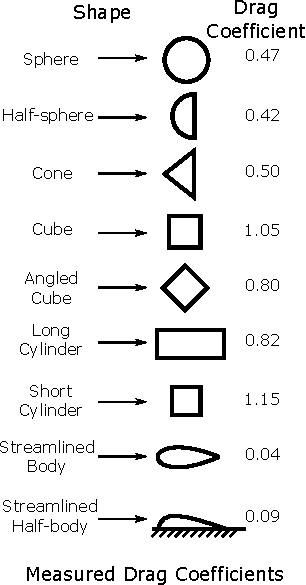
\includegraphics{Mechanical-Systems/drag-coefficient.pdf}
                }
            \end{center}
        \end{minipage}
        \vspace{-0.5em}
    \subsubsection{Conservative Forces}
        $
            F = - \grad U %- \frac{\partial U^T}{\partial q}
        $ : gradient of a potential function
       
    \subsection{Euler Method}
        \vspace{-1em}
        \begin{align*}
            E(t) &= T(t) + U(t) &\quad \frac{d}{dt}E(t) &= \sum_{i=1}^k P_i(t)
        \end{align*}

        \begin{itemize}
            \item  \textbf{Power $P$ of a Force}: \phantom{o} \boxed{P_F = \vec{F} \cdot \vec{v}}
            \item  \textbf{Power $P$ of a Torque}: \boxed{P_T = \vec{T} \cdot \vec{\omega}}
        \end{itemize}
    
       

            
            
